\documentclass[12pt]{article}
\usepackage[spanish]{babel}
\usepackage{graphicx}
\usepackage{float}

\title{Síntesis de redes activas \\ Laboratorio Nº3:Diseño de amplificadores}

\author{Profesor Titular: Dr. Ing. Pablo Ferreyra \\  Profesor Adjunto: Ing. César Reale \\ Alumnos: Campos Mariano, 
	Enzo Verstraete}

\begin{document}
	\maketitle
	
	\begin{abstract}
	Diseñar amplificadores utilizando tecnologías VFA y CFA, aplicando conceptos de compensación.
	\end{abstract}
	\newpage
	
	\section{Metodología}
	En general, para cada uno de los casos particulares solicitados, se debe:
	A. Realizar una sintética introducción teórica.
	B. Analizar el circuito propuesto, su desarrollo numérico, todos los cálculos analíticos.
	C. Realizar simulación en LTSPICE.
	D. Armar el circuito y hacer las mediciones en laboratorio.
	E. Finalmente comparar los valores calculados, simulados y medidos, y extraer conclusiones a
	cerca de las diferencias. Analizar las causas.
	F. Presentar un informe digital y en papel.
	
	\section{Desarrollo}
	La figura 1 muestran un amplificador compuesto que deberá ser diseñado para obtener una
	ganancia global Avf = 20dB, compensándolo para obtener una máxima planicidad de módulo
	(Mf = 65º o Qp = 0,707).
	
	\subsection{Configuración: 1.A VFA+VFA}
	Utilizando tecnologías VFA + VFA. Como amplificador VFA se utilizará un LM324, de 2(dos)
	polos (Ad0 = 100dB, FT = 1MHz, F1 = 10Hz y F2 = 5,06MHz).
	A.1 . Diseñar el amplificador compuesto VFA + VFA.
	A.2 . Calcular el ancho de banda potencial, la frecuencia del polo de la función de transferencia
	a lazo cerrado y ancho de banda a -3dB.
	A.3 Medir el ancho de banda a -3dB.
	A.4 . Estimar el margen de fase obtenido en base a la respuesta al escalón del amplificador
	compuesto.
	
	\begin{figure}[h!]
		\includegraphics[width=1\linewidth]{"D:/GD/Sintesis de redes activas/sintesis_redes_activas/Tp3/Simulaciones_Imagenes/1.A_Circ"}
		\caption[Amplificador configuración VFA+VFA]{Amplificador configuración VFA+VFA}
		\label{fig:1}
	\end{figure}
	
	Ganancia considerando el segundo amplificador operacional ideal, la ganancia a lazo abierto resulta:
	\begin{equation}
		\frac{V_{OUT}}{v_{IN}}=A_{D01}\frac{R1+R2}{R1}
	\end{equation}
	
	Ganancia de lazo:
	\begin{equation}
		\frac{V_{OUT}}{V_{VO'}}=\frac{Ri}{Ri+Rf}-A_{D01}\frac{R1+R2}{R1}
	\end{equation}
	
	Ganancia a lazo cerrado:
	\begin{equation}
		Avf=\frac{Av}{1-T}=\frac{A_{D01}\frac{R1+R2}{R1}}{1+\frac{Ri}{Ri+Rf}A_{D01}\frac{R1+R2}{R1}}
	\end{equation}
	
	Como $A_{D01}$ tiende a infinito, la ecuación se simplifica a la siguiente:
	\begin{equation}
			Avf=\frac{Av}{1-T}=\frac{Ri+Rf}{Ri}=10
	\end{equation}
	
	Seleccionamos los valores de resistencias para obtener el valor deseado $Ri=1[Kohm]$ y $Rf=9[Kohm]$
	
	El ancho de banda potencial $fg$ también se vincula con la ganancia del segundo operacional, buscando la condición de máxima planicidad del modulo tenemos la siguiente expresión:
	\begin{equation}
		M\Phi =180º -arctg\left( \frac{fg}{f1}\right) -arctg\left( \frac{fg}{f2}\right) =65.5º
	\end{equation}
	
	Con
	\begin{equation}
		arctg\left( \frac{fg}{f1}\right) =90º
	\end{equation}
	
	Por lo tanto 
	\begin{equation}
		fg=f2 tg\left( 24.5º)\right)=2.306[MHz]
	\end{equation}
	
	Con este valor determinamos la ganancia de lazo cerrado del segundo operacional
	
	\begin{equation}
		Avf2= \frac{Avf wg}{A_{D0} w1}=23
	\end{equation}
	
	Luego la ganancia a lazo abierto del amplificador compuesto resulta:
	\begin{equation}
		Avcomp=A_{D01}Avf2=2300000=127.24[dB]
	\end{equation}
	
	Calculamos los valores de R1 y R2:
	\begin{equation}
		R1=[1Kohm], R2=22[Kohm]
	\end{equation}
	
	\begin{figure}[h!]
		\includegraphics[width=1\linewidth]{"D:/GD/Sintesis de redes activas/sintesis_redes_activas/Tp3/Simulaciones_Imagenes/1.A_Sim_gain"}
		\caption[Salida del amplificador]{Salida del amplificador}
		\label{fig:2}
	\end{figure}
	
	\begin{figure}
		\includegraphics[width=1\linewidth]{"D:/GD/Sintesis de redes activas/sintesis_redes_activas/Tp3/Simulaciones_Imagenes/1.A_Frec_Resp"}
		\caption[Respuesta en frecuencia]{Respuesta en frecuencia}
		\label{fig:3}
	\end{figure}
	
	\subsection{Configuración: 1.B VFA+CFA}
	Utilizando tecnologías VFA + CFA. Se sugiere como amplificador VFA un LM324, de 2(dos)
	polos (Ad0 = 100dB, FT = 1MHz, F1 = 10Hz y F2 = 5,06MHz) y como CFA un LM6181 con RT =
	2,37M, CT = 4,8pF, cuya transimpedancia ZT presenta también 2(dos) polos (F1 = 14KHz, F2 =
	82,3MHz).
	B.1 . Diseñar el amplificador compuesto VFA + CFA para máxima planicidad de módulo y que
	además cumpla con un ancho de banda potencial aproximado de fg = 2MHz. Tener en
	cuenta la presencia del segundo polo del VFA.
	B.2 . Calcular el ancho de banda potencial, la frecuencia del polo de la función de transferencia
	a lazo cerrado y ancho de banda a -3dB.
	B.3 Medir el ancho de banda a -3dB.
	B.4 . Estimar el margen de fase obtenido en base a la respuesta al escalón del amplificador
	compuesto.
	
	\begin{figure}[h!]
		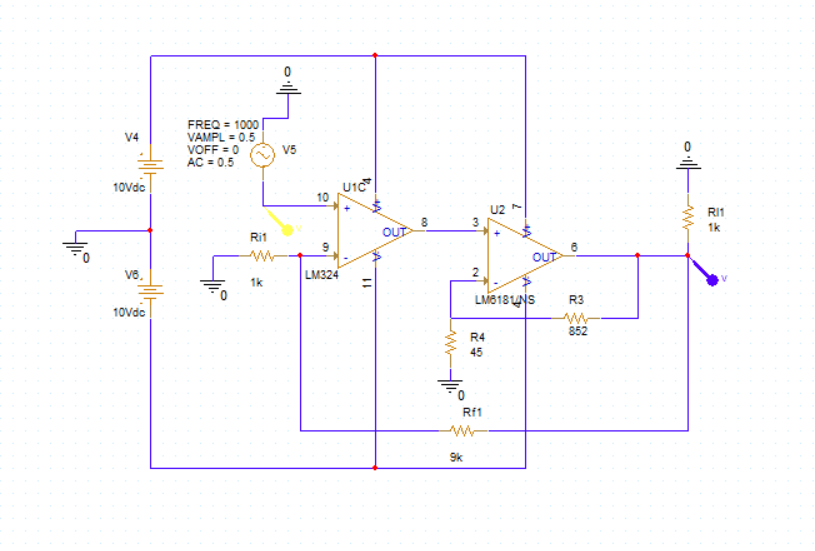
\includegraphics[width=1\linewidth]{Simulaciones_Imagenes/1.B_Circ}
		\caption[Amplificador configuración VFA+CFA]{Amplificador configuración VFA+CFA}
		\label{fig:4}
	\end{figure}
	
	Para $f2_{CFA}$ se considera que esta lo suficientemente alejado y VFA tiene el mismo comportamiento
	\begin{equation}
			M\Phi =180º-artg\left( \frac{fg}{f1_{VFA}}\right) -arctg\left( \frac{fg}{f2_{VFA}}\right) -arctg\left( \frac{fg}{f1_{CFA}}\right)=65.5º
	\end{equation} 
	
	\begin{equation}
		arctg\left( \frac{fg}{f1_{VFA}}\right) =90º
	\end{equation}
	
	\begin{equation}
		arctg\left( \frac{fg}{f2_{VFA}}\right) =21.56º
	\end{equation}
	
	\begin{equation}
		f_{CFA}= \frac{fg}{tg(2.94)}=38.9[MHz]
	\end{equation}
	
	Sabiendo que:
	\begin{equation}
		w_{CFA}=\frac{1}{CTR2}
	\end{equation}
	
	Calculamos el valor de R2:
	\begin{equation}
		R2=\frac{1}{CT 2 \pi f_{CFA}}=853[ohm]
	\end{equation}
	
	Teniendo en cuenta que el producto de ganancia por ancho de banda:
	\begin{equation}
		Avf fg = A_{D01}f1Avf2
	\end{equation}
	
	\begin{equation}
		Avf2=\frac{Avf fg}{A_{D01}f1} = \frac{R1+R2}{R1}=20
	\end{equation}
	
	Por ultimo obtenemos el valor de R2 y R1
	\begin{equation}
		R2=853[ohm], R1=44.84[ohm]
	\end{equation}
	
	\begin{figure}[h!]
		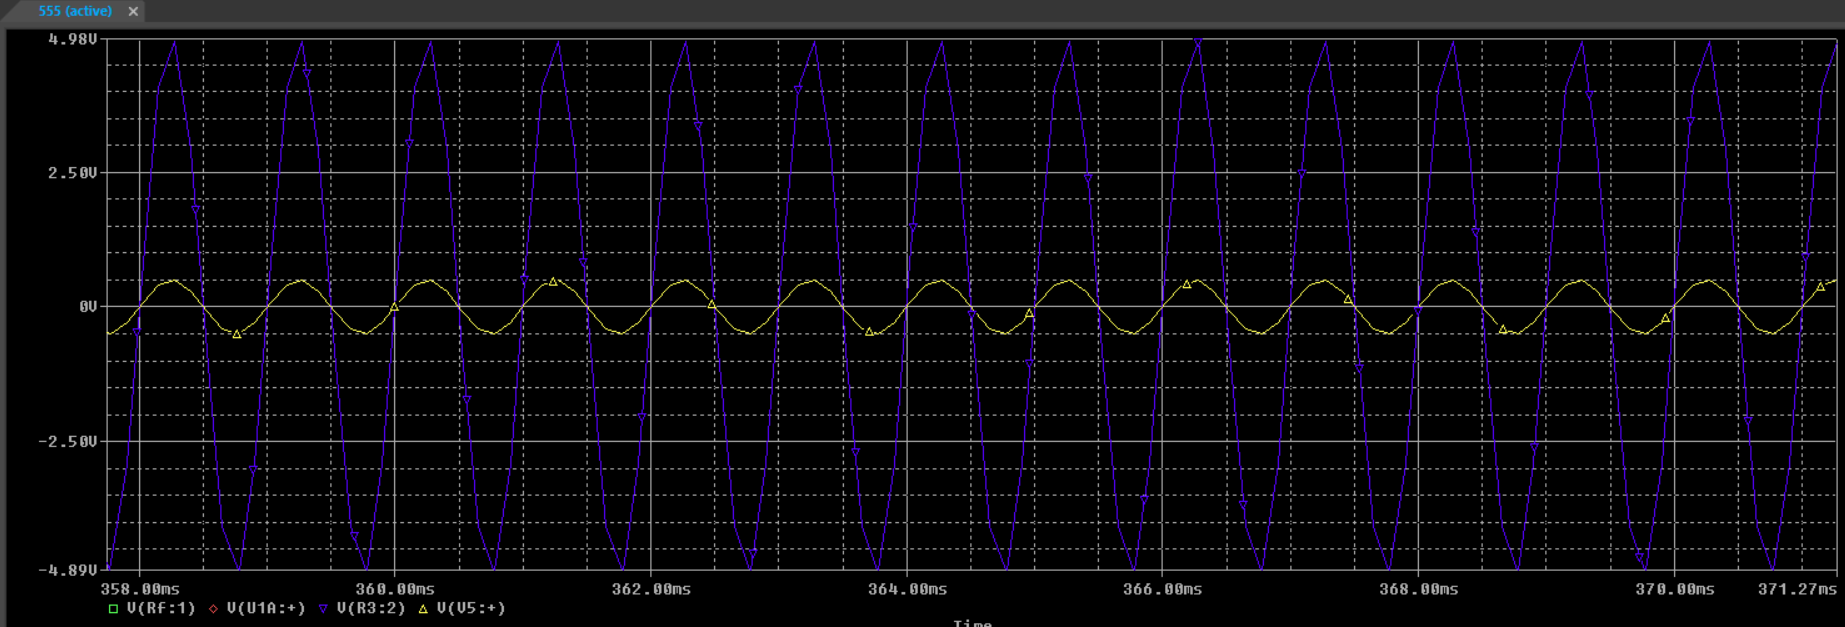
\includegraphics[width=1\linewidth]{Simulaciones_Imagenes/1.B_Sim_gain}
		\caption[Salida del amplificador]{Salida del amplificador}
		\label{fig:5}
	\end{figure}
	
	\begin{figure}[h!]
		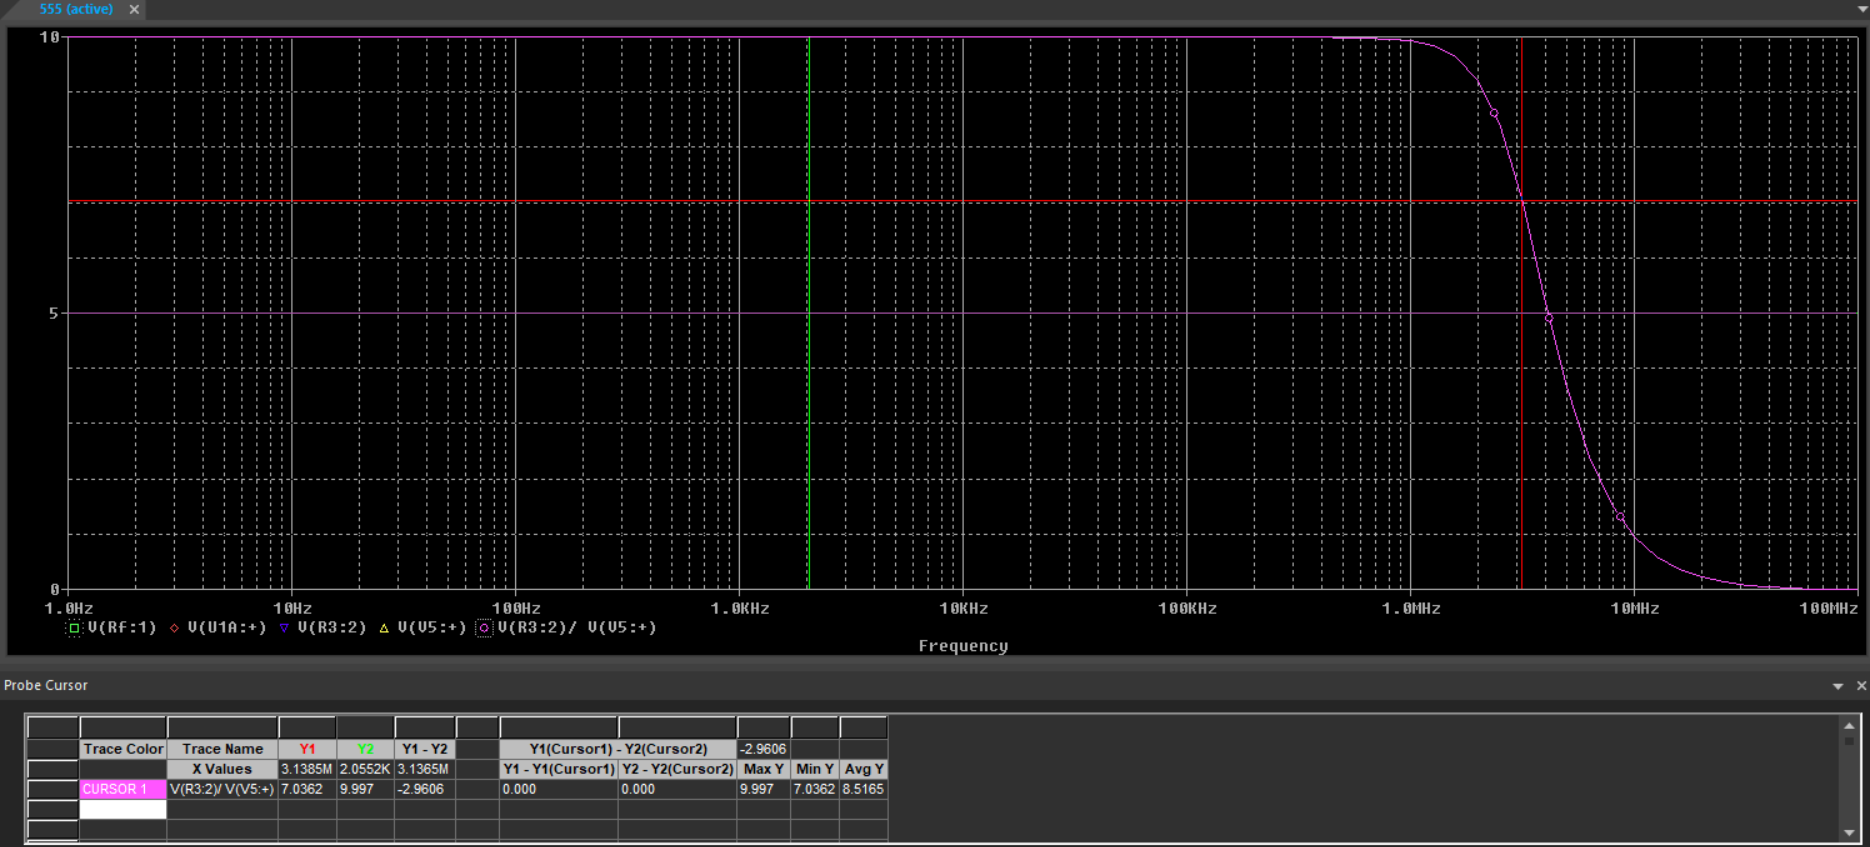
\includegraphics[width=1\linewidth]{Simulaciones_Imagenes/1.B_Frec_Resp}
		\caption[Respuesta en frecuencia]{Respuesta en frecuencia}
		\label{fig:6}
	\end{figure}
	
	\subsection{Configuración amplificador VFA+CFA II}
	Insertar en la configuración anterior una red de compensación cero – polo (a la salida del VFA)
	de tal modo que el cero de la red cancele el segundo polo del VFA. Ubicar el polo de la red a
	una octava de su cero. Retocar la ganancia del CFA realimentado para compensar la atenuación
	introducida por la red. Constatar la mejora del margen de fase a través de la respuesta al escalón.C.1 . Calcular y medir el margen de fase, el ancho de banda potencial, la frecuencia del polo de	la función de transferencia a lazo cerrado y ancho de banda a -3dB.
	C.2 . Calcular el ancho de banda potencial, la frecuencia del polo de la función de transferencia
	a lazo cerrado y ancho de banda a -3dB.
	C.3 Medir el ancho de banda a -3dB.
	C.4 . Estimar el margen de fase obtenido en base a la respuesta al escalón del amplificador
	compuesto.
	
	\begin{figure}
		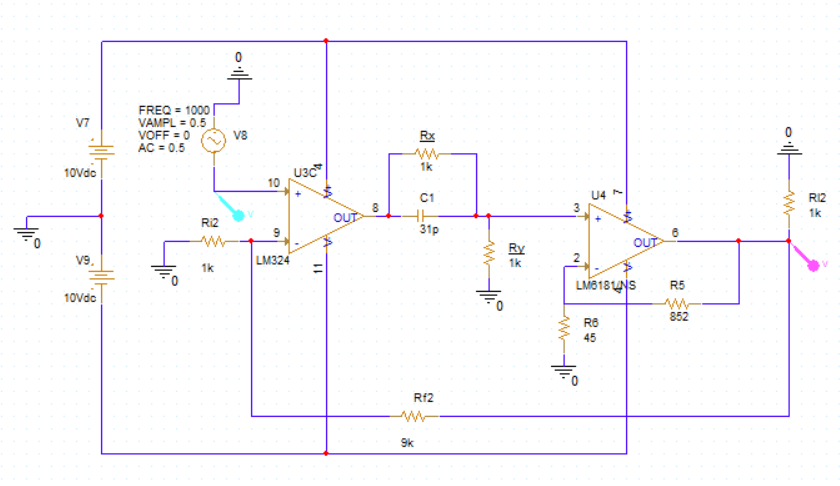
\includegraphics[width=1\linewidth]{Simulaciones_Imagenes/1.C_Circ}
		\caption[Diseño del compensador]{Diseño del compensador}
		\label{fig:7}
	\end{figure}
	
	Utilizamos una red de compensación cero-polo para cancelar el polo $f2_{VFA}$ y el polo del compensador se coloca a una octava de f2
	
	\begin{equation}
		w_{PC}=\frac{1}{Cx Rx//Ry}
	\end{equation}
	
	\begin{equation}
		w_{ZC}=\frac{1}{Cx Rx}
	\end{equation}
	
	La función de transferencia del compensador resulta:
	\begin{equation}
		Ac(s)=\frac{Ry}{Ry+Rx}\frac{1+sCxRx}{1+sCx(Rx//Ry)}
	\end{equation}
	
	\begin{equation}
			w_{ZC}=2 \pi f2[rps]
	\end{equation}
	\begin{equation}
		w_{PC}=2 \pi 10.12[Mrps]
	\end{equation}
	
	\begin{equation}
		2Ry=Rx+Ry=\frac{Rx}{Ry}=1
	\end{equation}
	Por lo tanto:
	\begin{equation}
		Rx=Ry=1[Kohm]
	\end{equation}
	
	\begin{equation}
		Cx=\frac{1}{w_{ZC}Rx}=\frac{1}{2 \pi f2 Rx}=3.15[pF]
	\end{equation}
	El compensador va despues del VFA por lo que hay que duplicar Avf2, entonces: $R2=852[ohm]$ y $\frac{R2}{R1}=39$, por lo tanto $R1=21.84[ohm]$
	
	\begin{figure}[h!]
		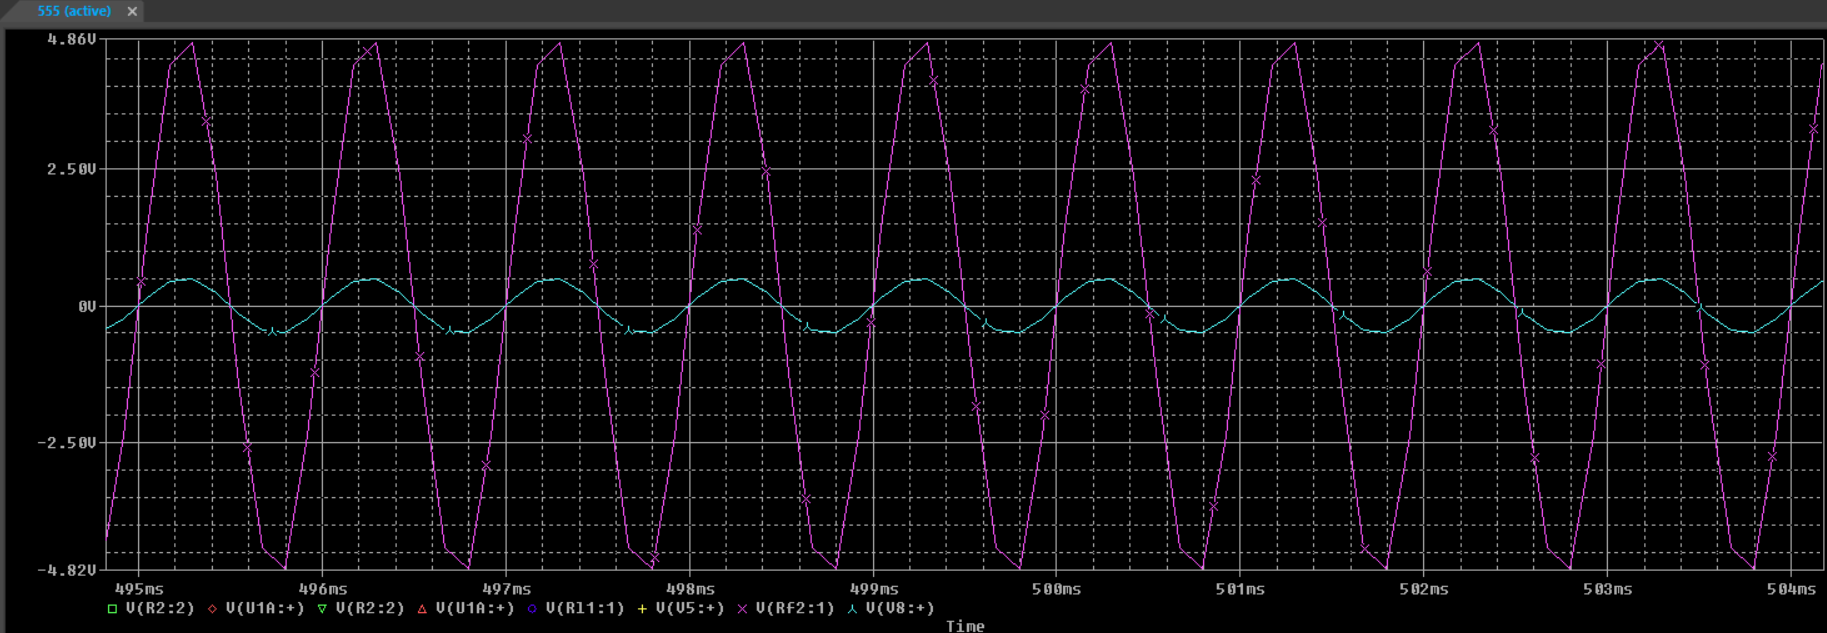
\includegraphics[width=1\linewidth]{Simulaciones_Imagenes/1.C_Sim_gain}
		\caption[Salida del amplificador]{Salida del amplificador}
		\label{fig:8}
	\end{figure}
	
	\begin{figure}[h!]
		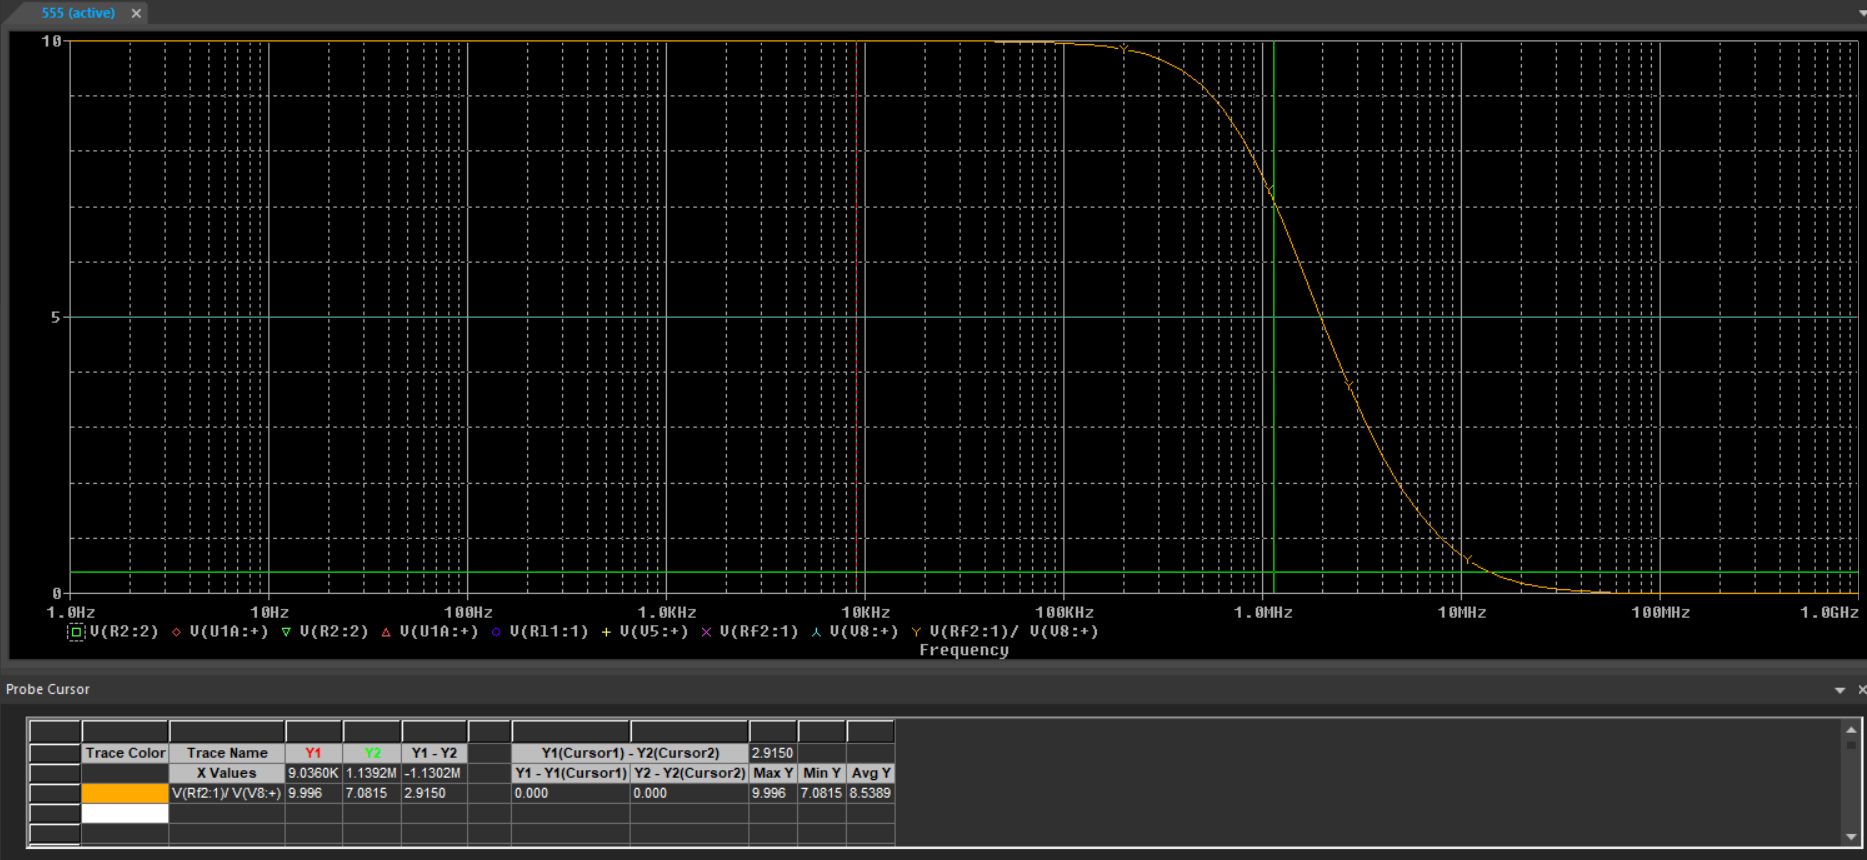
\includegraphics[width=1\linewidth]{Simulaciones_Imagenes/1.C_Frec_Resp}
		\caption[Respuesta en frecuencia]{Respuesta en frecuencia}
		\label{fig:9}
	\end{figure}
	
	
	
	
\end{document}
}